\documentclass[11pt, oneside]{article} 
\usepackage{geometry}
\geometry{letterpaper} 
\usepackage{graphicx}
	
\usepackage{amssymb}
\usepackage{amsmath}
\usepackage{parskip}
\usepackage{color}
\usepackage{hyperref}

\graphicspath{{/Users/telliott_admin/Dropbox/Github/Crypto/AES-math/}}
% \begin{center} \includegraphics [scale=0.4] {gauss3.png} \end{center}

\title{Galois fields like $GF(2^8)$}
\date{}

\begin{document}
\maketitle

\Large

\subsection*{Galois field}

For cryptography we process bytes (integers in the interval $[0,255]$.  The appropriate Galois field is called GF($2^8$).  We will use cofactors for the polynomials drawn from the set $\{0,1\}$ as before, but we go up to degree 7.

We will use an irreducible polynomial of degree 8 as the modulus.

We closed the last chapter by showing polynomials defined over $GF(2^3)$ modulo the irreducible polynomial $x^3 + x + 1$, which consist of the finite set:
\[ 0 \]
\[ 1 \]
\[ x \]
\[ x + 1 \]
\[ x^2 \]
\[ x^2 + 1 \]
\[ x^2 + x \]
\[ x^2 + x + 1 \]


Kak says:

\begin{quote} Our conceptualization of $GF(2^3)$ is analogous to our conceptualization of the set $Z_8$. The eight elements of $Z_8$ are to be thought of as integers modulo 8. So, basically, $Z_8$ maps all integers to the eight numbers in the set $Z_8$. Similarly, $GF(2^3)$maps all of the polynomials over $GF(2)$ to the eight polynomials shown above.\end{quote}

He continues:

\begin{quote}$GF(2^3)$ contains a unique multiplicative inverse for every non- zero element for the same reason that $Z_7$ contains a unique multiplicative inverse for every non-zero integer in the set. (For a counterexample, recall that $Z_8$ does not possess multiplicative inverses for 2, 4, and 6.) 

Stated formally, we say that for every non-zero element $a \in$ $GF(2^3)$ there is always a unique element $b \in$ $GF(2^3)$ such that $a \times b = 1$.

The above conclusion follows from the fact if you multiply a non-zero element $a$ with each of the eight elements of $GF(2^3)$, the result will be the eight distinct elements of $GF(2^3)$. 

Obviously, the results of such multiplications must equal 1 for exactly one of the non-zero elements of $GF(2^3)$. So if $a \times b = 1$, then $b$ must be the multiplicative inverse for $a$.

The same thing happens in $Z_7$. If you multiply a non-zero element $a$ of this set with each of the seven elements of $Z_7$, you will get seven distinct answers. The answer must therefore equal $1$ for at least one such multiplication. When the answer is $1$, you have your multiplicative inverse for $a$.\end{quote}.

In fact

\begin{quote}For a more formal proof (by contradiction) of the fact that if you multiply a non-zero element a of $GF(2^3)$ with every element of the same set, no two answers will be the same, let's assume that this assertion is false. That is, we assume the existence of two distinct values $b$ and $c$ in the set such that \end{quote}

\[ a \times b \equiv a \times c \mod (x^3 + x + 1) \]
which implies
\[ a \times (b - c) \equiv 0 \mod (x^3 + x + 1) \]
which implies either $a = 0$ or $b = c$, in either case this is a contradiction.

In exploring multiplication in $GF(2^8)$ constructed with the irreducible polynomial
\[ x^8 + x^4 + x^3 + x + 1 \]

My approach was to show by exhaustive search that every number has a unique multiplicative inverse, and furthermore for every product other than $1$ and every factor $a$ there is a unique $b$ such that $a \times b = p$.  We'll get to this later.

\subsection*{addition}

The fundamental definition of addition for our Galois field $GF(2^8)$  is that it is the same as the XOR operation:
\[ a \oplus b \]

Since $a \oplus a = 0$, it follows that each number is its own additive inverse, with a + a = 0.  Addition is the same as subtraction.  

And from this a clear implication is that multiplication is \emph{not} repeated addition.

The irreducible polynomial that is used for $GF(2^8)$ is
\[ x^8 + x^4 + x^3 + x + 1 \]

It is claimed that the finite field $GF(2^8)$ contains 256 distinct polynomials over $GF(2)$.

\subsection*{representations}

A common way to write numbers in $GF(2^8)$ is like this
\[ = x^7 + x^6 + x^5 + x^2 + x^1 + x^0 \]
the exponents on the last two terms are typically suppressed:
\[ =  x^7 + x^6 + x^5 + x^2 + x + 1 \]

If a term is present, then a $1$ is present in the place corresponding to the exponent, counting from right to left and starting with index 0. So

\[ x^7 + x^6 + x^5 + x^2 + x + 1 \]

is the same as binary $1110 \  \  0111$ or \textbf{0xe7}.  In fact, exactly the integers 0-255 or hex \textbf{00} to \textbf{ff} are in this field.

\subsection*{multiplication}

Multiplication by 1 is the easiest:  $b * 1 = b$, which is a great relief.

Multiplication by any number $\ge 2$ consists of two steps:  the multiplication itself, possibly followed by a mod operation.

\subsection*{multiplication by 2}

For multiplication by 2 there are two cases:  if the most significant bit (MSB) of $b$ is not set ($b \le 127$) then we simply do a left-shift:  throw away the left-hand 0 bit from $b$ and insert a $0$ bit on the right
\[ 0111 \  \  1111 * 2 =  1111 \  \  1110 = b' \]

If $b$ \emph{does} have its most-significant bit set ($b > 127$), then after the shift, we do the mod operation, which can be achieved by XOR with 27 ($ = 0001\ 1011$)	:
\[ b' \oplus 27 \]

We show later why this works later.  For now, move on to higher powers.

\subsection*{multiplication by powers of 2}

To multiply by 4 simply carry out two successive multiplications by 2.
\[ b * 4 = (b * 2) * 2 \]

For higher powers, lather, rinse and repeat:

\[ b * 8 = (b * 4) * 2 = ((b * 2) * 2) * 2 \]

\subsection*{multiplication by any number in GF($2^8$)}
Suppose we want to multiply $ 1000 \  \  0011 * b$.  First use the distributive law to write
\[ 1000 \   0011 * b \]
\[ = \ [ \ 1000 \   0000  + 0000 \  0010  + 0000 \   0001 \ ] \ * b \]
\[ = 1000 \  0000 * b + 0000 \  0010 * b + 0000 \  0001 * b \]
Break the multiplier into its constituent powers of two, multiply as before, and then carry out a final  addition step (which is just $\oplus$).

And that is really all we need.

When we understand the theory better, we hope to be able to explain why multiplying a 4-byte sequence like \textbf{db 13 53 45} by the matrix below to yield \textbf{8e 4d a1 bc} 

\[ fM =
\begin{bmatrix}
2 & 3 & 1 & 1 \\
1 & 2 & 3 & 1 \\
1 & 1 & 2 & 3 \\
3 & 1 & 1 & 2
\end{bmatrix} 
*
\begin{bmatrix}
db \\
13 \\
53 \\
45
\end{bmatrix} 
=
\begin{bmatrix}
8e \\
4d \\
a1 \\
bc
\end{bmatrix} 
\]


is reversed by multiplying the latter by

\[ rM = 
\begin{bmatrix}
14 &11 &13 & 9 \\
9 &14 &11 & 13 \\
13 & 9 &14 & 11 \\
11 &13 & 9 & 14
\end{bmatrix} \]

The reason is that 
\[ fM \times fM = rM \]
and
\[ fM \times fM \times fM = fM \times rM = I \]

And I wrote a matrix multiplication routine to prove it.

\subsection*{More about Galois Field math}

I found some other write-ups that provide a different perspective and a little more insight.

\url{http://www.cs.utsa.edu/~wagner/laws/FFM.html)}

Consider this multiplication: \textbf{ 0xb6 * 0x53}.  Write it in binary as:

\[ 1011\ 0110\ * \ 0101\ 0011 \]

We adopt a new notation.  Rewrite this as

\texttt{(7\ 5\ 4\ 2\ 1) * (6\ 4\ 1\ 0)}

This is a shorthand version of the Galois field notation:

\[ (x^7 + x^5 + x^4 + x^2 + x) * (x^6 + x^4 + x + 1) \]

The first line below restates the problem, then we do the multiplication one digit at a time.  It turns out that we can multiply by each of the digits, XOR the result, and not worry about the mod until the end.

\begin{center} 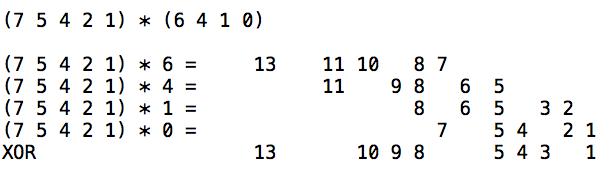
\includegraphics [scale=0.6] {figs/GFmath1.png} \end{center}

Recall above where we said that multiplying by decimal 2, which is the same as multiplying by $x$ in the field notation, is also the same as a left-shift of 1 in the binary representation.  In the line $(7 \ 5 \ 4 \ 2 \ 1) * 6$, we simply add $6$ to each of the digits in the first number to give the result (13,11,10,8,7).  The spacing is used to simplify the XOR on the last line.

Now, we do the mod operation.
\begin{center} 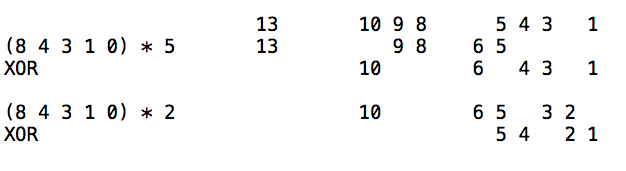
\includegraphics [scale=0.6] {figs/GFmath2.png} \end{center}
The special divisor is $(8,4,3,1,0)$. 
\[ (x^8 + x^4 + x^3 + x + 1) \]

We multiply by $5$ to get it to align with the $13$ in the interim result.  This is the same as multiplying the irreducible polynomial by $x^5$ or multiplying its binary equivalent (1 0001 1011) by $2^5$.

After the XOR, the $13$ is gone.  We repeat the process, lining up with the $10$ and zeroing it out.  If there had been an $8$ we would go that far, but no farther.

Our answer, then, is $0011 \ 0110$ which is \textbf{0x36}.

The complete multiplication is:  \textbf{0xb6 * 0x53 = 0x36}.

Effectively what we've done is to do repeated divisions by powers of two of the super duper special number (1 0001 1011).  We guarantee that every place higher than $8$ will be turned to zero by this operation.

\subsection*{wikipedia example}

Another view of the modulus or division operation comes from the wikipedia example:  \textbf{0x53 * 0xca}.  We write this in binary:  $0101 \ 0011 \ * \ 1100 \ 1010$.

In our new notation, this would be

\begin{center} 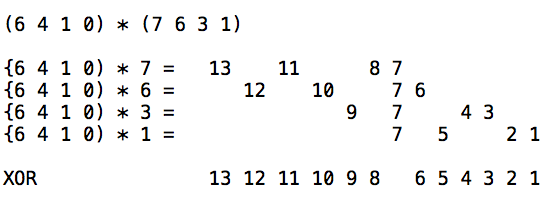
\includegraphics [scale=0.6] {figs/GFmath3.png} \end{center}
which looks like it's pretty special.  And it is. 

 Here is the mod step:
\begin{center} 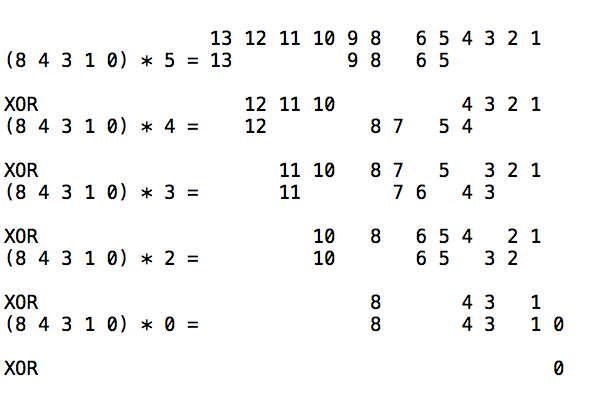
\includegraphics [scale=0.6] {figs/GFmath4.png} \end{center}

That $0$ at the end is not really zero.  It is a power of $2$, or $2^0 =$ \textbf{0x01}.  What we've shown is that  \textbf{0x53 * 0xca = 0x01}.  In other words, \textbf{0x53} is the \emph{multiplicative inverse} of \textbf{0xca}.

Let's take a look at doing the same mod operation as long division, which should hammer  home the point we've been absorbing.
\begin{center} 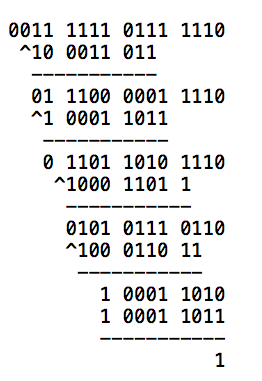
\includegraphics [scale=0.6] {figs/GFmath5.png} \end{center}

\subsection*{extended Euclidean algorithm}
It is possible to apply the "extended" Euclidean algorithm to the problem of finding multiplicative inverses.  We developed this topic in the write-up on GF($2^3$).  The calculations for GF($2^8$) are a bit hairier, but it seems to work as it should .  Here is one example:

\begin{verbatim}
100011011 is the irreducible polynomial

consider 
x^6 + x^3 + x + 1 = 1001011
we need 2 places thus q = 100
ignore the rest

a          b        q    qb
100011011  1001011  100  100101100
 
100011011
100101100
---------
   110111

a        b       q   qb
1001011  110111  11  1011001

1001011
1011001
-------
  10010

a       b      q   qb
110111  10010  11  110110
110110
------
     1

Backtrack:

110111 = 100011011 - 100 * 1001011
 10010 =   1001011 -  11 *  110111
     1 =    110111 -  11 *   10010

     1 =    110111 -  11 * [1001011 -  11 *  110111]
       = 100 * 110111 - 11 * 1001011
       = 100 [100011011 - 100 * 1001011] - 11 * 1001011
       = -10000 * 1001011 - 11 * 1001011
       = (10011) * 1001011
       = (x^4 + x + 1)(x^6 + x^3 + x + 1)

Check

(x^4 + x + 1)(x^6 + x^3 + x + 1)
= x^10 + x^7 + x^7 + x^6 + x^5 + x^4 + x^4 + x^3 + x^2 + x + x + 1
= x^10 + x^6 + x^5 + x^3 + x^2 + 1
= 100 0110 1001

mod
100 0110 1101
100 0110 11
-------------
            1
\end{verbatim}
            
We calculate that $(x^4 + x + 1)(x^6 + x^3 + x + 1) = 1$

In hex, that's \textbf{13} * \textbf{4b} = \textbf{01}.  If you check the table of multiplicative inverses, you'll see that's a match.

I don't care to do any more!

\end{document}